This section is concerned with the appendices of the WorkSheets

\subsection{PumpCoefficients} \label{ap:PumpCoef}

A model of the pump is based on the following relationship between the pressure drop over the pump and the pump speed, flow through the pump and the pump coefficients.

The full pump model:
\begin{equation} \label{eq:pumpmodel}
		\Delta p_{pump}  = a_0  \cdot \omega^2 + a_1 \cdot q \cdot \omega + a_2 \cdot q^2
\end{equation}

The pump coefficients are estimated from the pump performance curves from the data-sheets. These describe the exact relationship described in \cref{eq:pumpmodel}.

The preassure drops were read at the following flows:

\begin{equation}
	q = \begin{bmatrix}
		0 & 0.5 & 1 & 1.5 & 2 & 2.5 & 3 & 3.5 
	\end{bmatrix} 
\label{eq:pump_q}
\end{equation}

At these flows the pressure drop across the pump were read from the y-axis at three different pump speeds, namely 80\%, 69\% and 48\%. The recorded pressure drops were the following:

\begin{equation}
	p =  \begin{bmatrix}
		p_{80}\\
		p_{69} \\
		p_{48}
	\end{bmatrix}  = 
	\begin{bmatrix}
		5.57 & 5.85 & 5.9 & 5.7 & 5.1 & 4.25 & 3.3 & 2.4 \\
		4.1 & 4.2 & 4.2 & 4 & 3.55 & 3 & 2.3 & 1.55 \\
		1.75 & 1.85 & 1.7 & 1.3 & 0.95 &  &  &  
	\end{bmatrix} 
\label{eq:pump_p}
\end{equation}

Only 5 pressure readings were made from the 48\% pump speed.

The coefficients are found by finding the leas square solution to following equation:

\begin{equation}
	Ax = b \leftrightarrow x = (A^TA)^{-1}A^Tb
\end{equation}
where A is a matrix defined as follows:
\begin{equation}
	A = \begin{bmatrix}
			\omega^2 & q \cdot \omega & q^2
			\end{bmatrix}
\end{equation}

With number of rows corresponding to the amount of data points in $ p $, i.e. the for 8 rows corresponds to measurements made for $ \omega = 80$, the next 8 rows corresponds to measurements made for $ \omega = 69 $ etc.  

and $ b = \begin{bmatrix}
	p_{80} \hspace{0.3cm} p_{69} \hspace{0.3cm} p_{48}
\end{bmatrix} $$ ^T $ from \cref{eq:pump_p}.

The solution yields the following coefficients:
\begin{equation}
	\begin{split}
		a_0 = 0.0001 \\
		a_1 = 0.0004 \\
		a_2 = -0.0323 \\
	\end{split}
\end{equation}

We confirm our pump model by comparing it to actual data points on the pump curve from the data sheet.
\begin{figure}[h!]
	\centering
	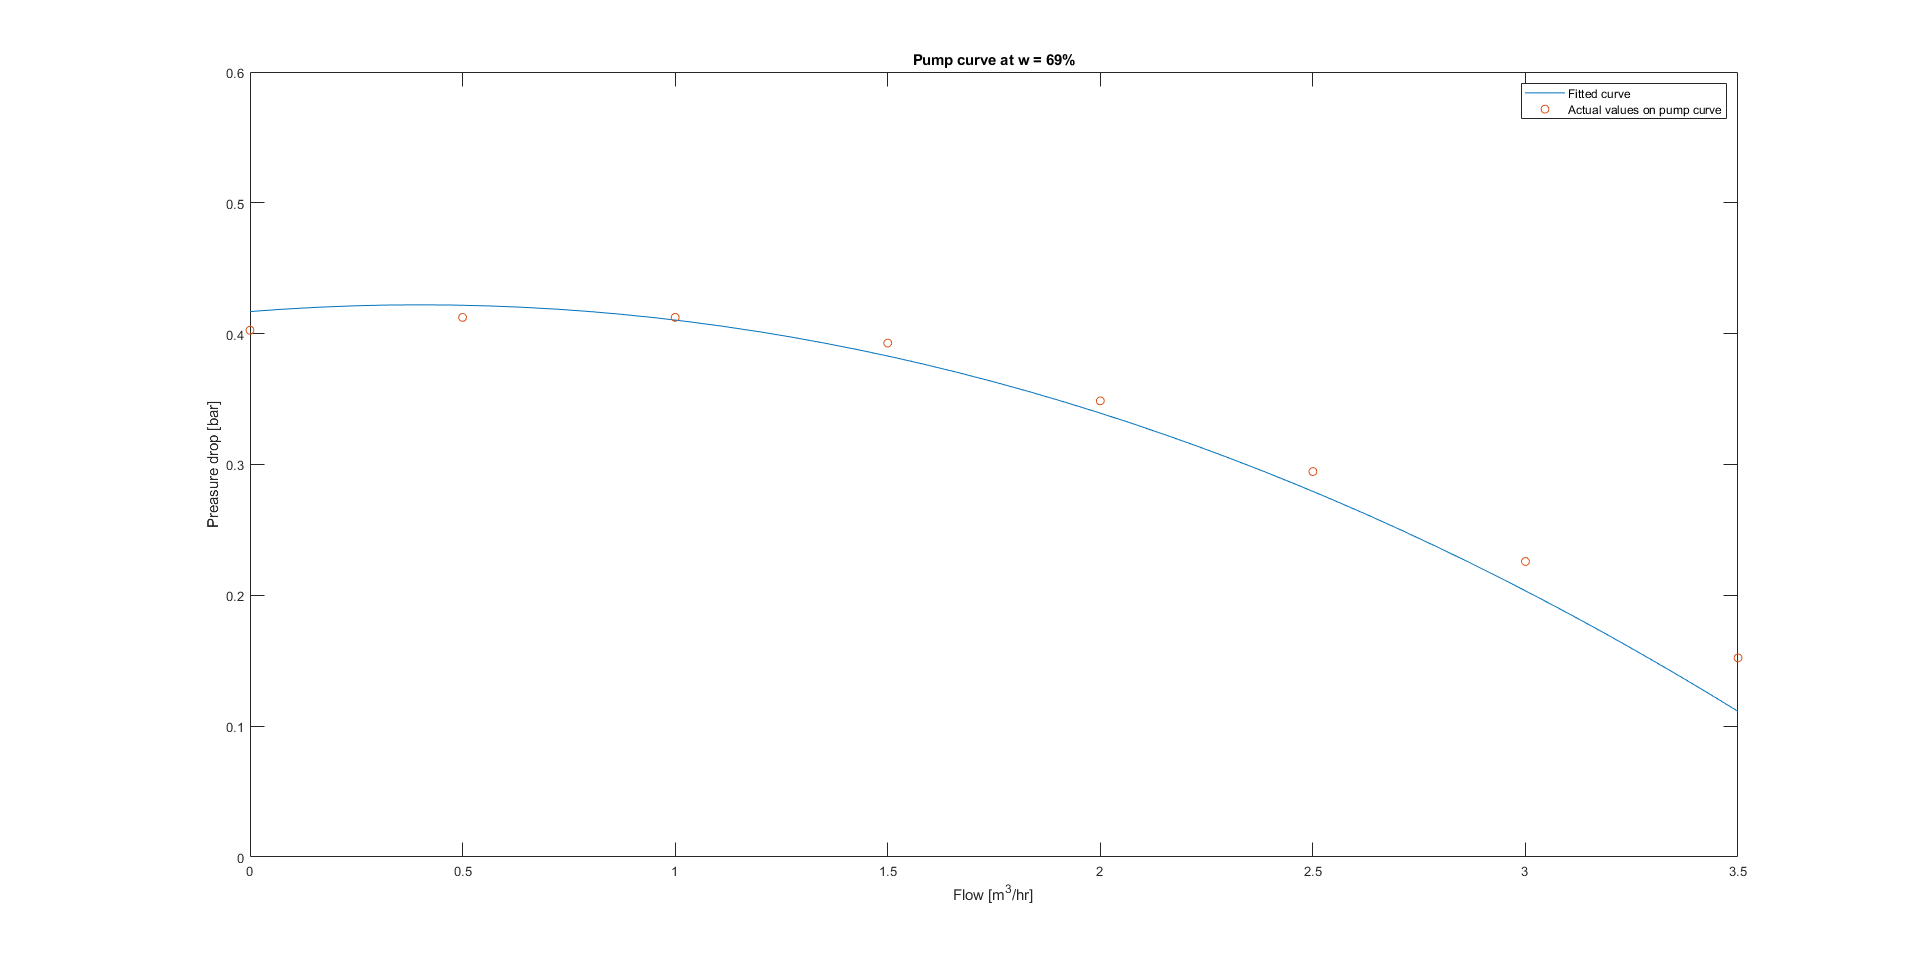
\includegraphics[width=0.7\textwidth]{Pictures/Pumpcurve_69.png}
	\caption{Comparing model of pump curve with actual values from data sheet}
	\label{fig:Pumpcurve_69}
\end{figure}








